\documentclass{jlreq}

\usepackage{titlesec}
\usepackage{listings}
\usepackage{fancyhdr}

% \adjustbox
\usepackage{adjustbox}

% tcolorboxの設定
\usepackage[most]{tcolorbox} 
\tcbuselibrary{breakable}
\tcbuselibrary{skins}
\tcbuselibrary{listingsutf8}
% タイトルのフォーマットを変更
\titleformat{\title}
  {\centering\Huge\bfseries}
  {}
  {0em} 
  {}

\titleformat{\subtitle}
  {\centering\Large\itshape}
  {}
  {0em}
  {}

\titleformat{\subsubsection}[block]
  {\normalfont\normalsize\bfseries}
  {\arabic{subsubsection}.}
  {1em}
  {}

\titleformat{\section}[block]
  {\normalfont\large\bfseries}
  {\Roman{section}.}
  {1em} 
  {}
  [\titleline{\titlerule[1pt]}]

\titleformat{\subsection}[block]
  {\normalfont\normalsize\bfseries}
  {\roman{subsection}.}
  {1em}
  {}

% listingsの設定

\renewcommand{\lstlistingname}{コード}

\lstset{
	breaklines = true,
	language = Python,
	keywordstyle = {\bfseries \color[cmyk]{0,1,0,0}},
	commentstyle = {\itshape \color[cmyk]{1,0.4,1,0}},
	numbers = left,
	numberstyle = \tiny,
	stepnumber = 1,
	% frameとnumberの間の距離
	numbersep = 10pt,
	frame = single,
	basicstyle = \ttfamily,
	tabsize = 2,
	captionpos = t,
	backgroundcolor={\color[gray]{.90}},
	showstringspaces = false,
}

% headerの設定
\pagestyle{fancy}
\fancyhf{}

\fancyhead[RO,RE]{\rightmark}
\fancyhead[LO,LE]{\leftmark} 
\fancyfoot[C]{\thepage}

% tikzの設定
\usepackage{tikz}

\begin{document}

EEIC2024アルゴリズムの授業で扱った文字列照合のアルゴリズムのシケプリです。扱った内容は以下の通りです。
\begin{itemize}
	\item 力任せ法
	\item KMP法
	\item BM法
    \item BMH法
	\item ラビン・カープ法(ローリングハッシュ)
\end{itemize}

\section{力任せ法}
力任せ法は文字通り文字列において、所望のパターンが見つかるまで前から順に比較していく方法です。
以下でtextとpatternの文字列が与えられたときに、textの中にpatternが含まれるかどうか考えましょう。文字列の文字を表す記法は
text[i]のように0-indexで表します。

最初はtext[0]とpattern[0]を比較すると一致しません。一致しないときは、textのcursorを1つ進めてtext[1]とpattern[0]を比較します。

\vspace{0.5cm}
\begin{center}
    \begin{tabular}{|c|c|c|c|c|c|c|c|c|c|c|c|c|}
        \hline
		\makebox[0.5cm]{B} & \makebox[0.5cm]{A} & \makebox[0.5cm]{B} & \makebox[0.5cm]{A} & \makebox[0.5cm]{B} & \makebox[0.5cm]{C} & \makebox[0.5cm]{B} & \makebox[0.5cm]{A} & \makebox[0.5cm]{B} & \makebox[0.5cm]{A} & \makebox[0.5cm]{B} & \makebox[0.5cm]{D} & \makebox[0.5cm]{B} \\ 
        \hline
    \end{tabular}
\end{center}
\begin{center}
    text
\end{center}

\vspace{0.5cm}

% セルの幅を統一した二つ目の表
\begin{center}
    \begin{tabular}{|c|c|c|c|c|c|c|c|c|c|c|c|c|}
        \hline
        \makebox[0.5cm]{A} & \makebox[0.5cm]{B} & \makebox[0.5cm]{A} & \makebox[0.5cm]{B} & \makebox[0.5cm]{D} & \makebox[0.5cm]{} & \makebox[0.5cm]{} & \makebox[0.5cm]{} & \makebox[0.5cm]{} & \makebox[0.5cm]{} & \makebox[0.5cm]{} & \makebox[0.5cm]{} & \makebox[0.5cm]{} \\ 
        \hline
    \end{tabular}
\end{center}
\begin{center}
    pattern
\end{center}

text[1]とpattern[0]を比較すると、一致します。しかし、text[5]とpattern[4]が一致しないので、textのcursorを1つ進めてtext[2]とpattern[0]を比較します。

\vspace{0.5cm}
\begin{center}
    \begin{tabular}{|c|c|c|c|c|c|c|c|c|c|c|c|c|}
        \hline
		\makebox[0.5cm]{B} & \makebox[0.5cm]{A} & \makebox[0.5cm]{B} & \makebox[0.5cm]{A} & \makebox[0.5cm]{B} & \makebox[0.5cm]{C} & \makebox[0.5cm]{B} & \makebox[0.5cm]{A} & \makebox[0.5cm]{B} & \makebox[0.5cm]{A} & \makebox[0.5cm]{B} & \makebox[0.5cm]{D} & \makebox[0.5cm]{B} \\ 
        \hline
    \end{tabular}
\end{center}
\begin{center}
    text
\end{center}

\vspace{0.5cm}

% セルの幅を統一した二つ目の表
\begin{center}
    \begin{tabular}{|c|c|c|c|c|c|c|c|c|c|c|c|c|}
        \hline
        \makebox[0.5cm]{} & \makebox[0.5cm]{A} & \makebox[0.5cm]{B} & \makebox[0.5cm]{A} & \makebox[0.5cm]{B} & \makebox[0.5cm]{D} & \makebox[0.5cm]{} & \makebox[0.5cm]{} & \makebox[0.5cm]{} & \makebox[0.5cm]{} & \makebox[0.5cm]{} & \makebox[0.5cm]{} & \makebox[0.5cm]{} \\ 
        \hline
    \end{tabular}
\end{center}
\begin{center}
    pattern
\end{center}

これを一致していくまで続けていくと、以下のようになります。

\vspace{0.5cm}
\begin{center}
    \begin{tabular}{|c|c|c|c|c|c|c|c|c|c|c|c|c|}
        \hline
        \makebox[0.5cm]{B} & \makebox[0.5cm]{A} & \makebox[0.5cm]{B} & \makebox[0.5cm]{A} & \makebox[0.5cm]{B} & \makebox[0.5cm]{C} & \makebox[0.5cm]{B} & \makebox[0.5cm]{A} & \makebox[0.5cm]{B} & \makebox[0.5cm]{A} & \makebox[0.5cm]{B} & \makebox[0.5cm]{D} & \makebox[0.5cm]{B} \\ 
        \hline
    \end{tabular}
\end{center}
\begin{center}
    text
\end{center}

\vspace{0.5cm}

% セルの幅を統一した二つ目の表
\begin{center}
    \begin{tabular}{|c|c|c|c|c|c|c|c|c|c|c|c|c|}
        \hline
        \makebox[0.5cm]{} & \makebox[0.5cm]{} & \makebox[0.5cm]{} & \makebox[0.5cm]{} & \makebox[0.5cm]{} & \makebox[0.5cm]{} & \makebox[0.5cm]{} & \makebox[0.5cm]{A} & \makebox[0.5cm]{B} & \makebox[0.5cm]{A} & \makebox[0.5cm]{B} & \makebox[0.5cm]{D} & \makebox[0.5cm]{} \\ 
        \hline
    \end{tabular}
\end{center}
\begin{center}
    pattern
\end{center}

例を通じて力任せ法では、textを0からtextの長さ - patternの長さまで動かすことで、patternがtextに含まれるかどうかを判定することができます。C言語で
プログラムを書いてみましょう。

\begin{lstlisting}[]
	#include<stdio.h>
#include<string.h>

int brute_force(char text[], int text_size, char pattern[], int pattern_size) {
	/*
	力任せ法によって一致する場合はその位置を返し、一致しない場合は-1を返す
	args:
		text: 探索対象のテキスト
		text_size: textのサイズ
		pattern: 探索するパターン
		pattern_size: patternのサイズ
	*/

	for (int text_cursor = 0; text_cursor < text_size - pattern_size + 1; ++text_cursor) {
		int pattern_cursor = 0;

		while (pattern_cursor < pattern_size) {
			if (text[text_cursor + pattern_cursor] == pattern[pattern_cursor]) {
				++pattern_cursor;
			} else {
				break;
			}
		}

		if (pattern_cursor == pattern_size) {
			return text_cursor;
		}
	}
	return -1;
}

int main(int argc, char **argv) {
	char text[] = "BABABCBABABDB";
	char pattern[] = "ABABD";

	int matched_position = brute_force(text, strlen(text), pattern, strlen(pattern));

	if (matched_position == -1) {
		printf("not matched\n");
	} else {
		printf("matched at %d\n", matched_position);
	}

	return 0;
} 
\end{lstlisting}

\section{KMP法}
\subsection{力任せ法の無駄}
\vspace{0.5cm}
\begin{center}
    \begin{tabular}{|c|c|c|c|c|c|c|c|c|c|c|c|c|}
        \hline
		\makebox[0.5cm]{B} & \makebox[0.5cm]{A} & \makebox[0.5cm]{B} & \makebox[0.5cm]{A} & \makebox[0.5cm]{B} & \makebox[0.5cm]{C} & \makebox[0.5cm]{B} & \makebox[0.5cm]{A} & \makebox[0.5cm]{B} & \makebox[0.5cm]{A} & \makebox[0.5cm]{B} & \makebox[0.5cm]{D} & \makebox[0.5cm]{B} \\ 
        \hline
    \end{tabular}
    \begin{tikzpicture}[overlay, scale=0.5]
        \draw[->, thick] (-19.9, -2) -- (-19.9, -1.5);
    \end{tikzpicture}
\end{center}
\begin{center}
    text
\end{center}

\vspace{0.5cm}

% セルの幅を統一した二つ目の表
\begin{center}
    \begin{tabular}{|c|c|c|c|c|c|c|c|c|c|c|c|c|}
        \hline
        \makebox[0.5cm]{} & \makebox[0.5cm]{A} & \makebox[0.5cm]{B} & \makebox[0.5cm]{A} & \makebox[0.5cm]{B} & \makebox[0.5cm]{D} & \makebox[0.5cm]{} & \makebox[0.5cm]{} & \makebox[0.5cm]{} & \makebox[0.5cm]{} & \makebox[0.5cm]{} & \makebox[0.5cm]{} & \makebox[0.5cm]{} \\ 
        \hline
    \end{tabular}
\end{center}
\begin{center}
    pattern
\end{center}

\vspace{1cm}

上の例ではtext[1]から照合を始めてtext[5]で照合が失敗していることがわかります。力任せ法では
次にtext[2]から照合を始めることになりますが、それはtextの方のcursorが一度通った場所を再度通ることになります。このように、力任せ法は
textのcursorが一度通った場所を再び通ることが多いため、無駄が多いといえます。
ただ、上の例ではABABというパターンがあって、ABABの部分が繰り返されていることがわかります。このような繰り返し部分がある場合、
次に照合を始める位置をスキップすることで無駄が省けそうではないでしょうか?下の例では、textのcursorが後戻りすることなく、patternの位置も
前にスキップされています。

\vspace{0.5cm}
\begin{center}
    \begin{tabular}{|c|c|c|c|c|c|c|c|c|c|c|c|c|}
        \hline
		\makebox[0.5cm]{B} & \makebox[0.5cm]{A} & \makebox[0.5cm]{B} & \makebox[0.5cm]{A} & \makebox[0.5cm]{B} & \makebox[0.5cm]{C} & \makebox[0.5cm]{B} & \makebox[0.5cm]{A} & \makebox[0.5cm]{B} & \makebox[0.5cm]{A} & \makebox[0.5cm]{B} & \makebox[0.5cm]{D} & \makebox[0.5cm]{B} \\ 
        \hline
    \end{tabular}
    \begin{tikzpicture}[overlay, scale=0.5]
        \draw[->, thick] (-16.4, -2) -- (-16.4, -1.5);
    \end{tikzpicture}
\end{center}
\begin{center}
    text
\end{center}

\vspace{0.5cm}

% セルの幅を統一した二つ目の表
\begin{center}
    \begin{tabular}{|c|c|c|c|c|c|c|c|c|c|c|c|c|}
        \hline
        \makebox[0.5cm]{} & \makebox[0.5cm]{} & \makebox[0.5cm]{} & \makebox[0.5cm]{A} & \makebox[0.5cm]{B} & \makebox[0.5cm]{A} & \makebox[0.5cm]{B} & \makebox[0.5cm]{D} & \makebox[0.5cm]{} & \makebox[0.5cm]{} & \makebox[0.5cm]{} & \makebox[0.5cm]{} & \makebox[0.5cm]{} \\ 
        \hline
    \end{tabular}
\end{center}
\begin{center}
    pattern
\end{center}

\vspace{1cm}

\subsection{KMP法の仕組み}
上のスキップを実現する方法の1つにKMP法があります。KMP法の流れを具体例を見て確認します。

\vspace{0.5cm}
\begin{center}
    \begin{tabular}{|c|c|c|c|c|c|c|c|c|c|c|c|c|}
        \hline
		\makebox[0.5cm]{B} & \makebox[0.5cm]{A} & \makebox[0.5cm]{B} & \makebox[0.5cm]{A} & \makebox[0.5cm]{B} & \makebox[0.5cm]{C} & \makebox[0.5cm]{B} & \makebox[0.5cm]{A} & \makebox[0.5cm]{B} & \makebox[0.5cm]{A} & \makebox[0.5cm]{B} & \makebox[0.5cm]{D} & \makebox[0.5cm]{B} \\ 
        \hline
    \end{tabular}
    \begin{tikzpicture}[overlay, scale=0.5]
        \draw[->, thick] (-13.1, -2) -- (-13.1, -1.5);
    \end{tikzpicture}
\end{center}
\begin{center}
    text
\end{center}

\vspace{0.5cm}

% セルの幅を統一した二つ目の表
\begin{center}
    \begin{tabular}{|c|c|c|c|c|c|c|c|c|c|c|c|c|}
        \hline
        \makebox[0.5cm]{} & \makebox[0.5cm]{A} & \makebox[0.5cm]{B} & \makebox[0.5cm]{A} & \makebox[0.5cm]{B} & \makebox[0.5cm]{D} & \makebox[0.5cm]{} & \makebox[0.5cm]{} & \makebox[0.5cm]{} & \makebox[0.5cm]{} & \makebox[0.5cm]{} & \makebox[0.5cm]{} & \makebox[0.5cm]{} \\ 
        \hline
    \end{tabular}
    \begin{tikzpicture}[overlay, scale=0.5]
        \draw[->, thick] (-13.1, -2) -- (-13.1, -1.5);
    \end{tikzpicture}
\end{center}
\begin{center}
    pattern
\end{center}

\vspace{0.5cm}

\begin{center}
    (1)
\end{center}

%%%%%%%%%%%%%%%%%%%%%%%%%%%%%%%%%%%%%%%%%%%%%%%%%%%%%%%%%%%%

\vspace{0.5cm}
\begin{center}
    \begin{tabular}{|c|c|c|c|c|c|c|c|c|c|c|c|c|}
        \hline
		\makebox[0.5cm]{B} & \makebox[0.5cm]{A} & \makebox[0.5cm]{B} & \makebox[0.5cm]{A} & \makebox[0.5cm]{B} & \makebox[0.5cm]{C} & \makebox[0.5cm]{B} & \makebox[0.5cm]{A} & \makebox[0.5cm]{B} & \makebox[0.5cm]{A} & \makebox[0.5cm]{B} & \makebox[0.5cm]{D} & \makebox[0.5cm]{B} \\ 
        \hline
    \end{tabular}
    \begin{tikzpicture}[overlay, scale=0.5]
        \draw[->, thick] (-13.1, -2) -- (-13.1, -1.5);
    \end{tikzpicture}
\end{center}
\begin{center}
    text
\end{center}

\vspace{0.5cm}

\begin{center}
    \begin{tabular}{|c|c|c|c|c|c|c|c|c|c|c|c|c|}
        \hline
        \makebox[0.5cm]{} & \makebox[0.5cm]{} & \makebox[0.5cm]{} & \makebox[0.5cm]{A} & \makebox[0.5cm]{B} & \makebox[0.5cm]{A} & \makebox[0.5cm]{B} & \makebox[0.5cm]{D} & \makebox[0.5cm]{} & \makebox[0.5cm]{} & \makebox[0.5cm]{} & \makebox[0.5cm]{} & \makebox[0.5cm]{} \\ 
        \hline
    \end{tabular}
    \begin{tikzpicture}[overlay, scale=0.5]
        \draw[->, thick] (-13.1, -2) -- (-13.1, -1.5);
    \end{tikzpicture}
\end{center}
\begin{center}
    pattern
\end{center}

\vspace{0.5cm}

\begin{center}
    (2)
\end{center}

\vspace{0.5cm}

%%%%%%%%%%%%%%%%%%%%%%%%%%%%%%%%%%%%%%%%%%%%%%%%%
\vspace{0.5cm}
\begin{center}
    \begin{tabular}{|c|c|c|c|c|c|c|c|c|c|c|c|c|}
        \hline
		\makebox[0.5cm]{B} & \makebox[0.5cm]{A} & \makebox[0.5cm]{B} & \makebox[0.5cm]{A} & \makebox[0.5cm]{B} & \makebox[0.5cm]{C} & \makebox[0.5cm]{B} & \makebox[0.5cm]{A} & \makebox[0.5cm]{B} & \makebox[0.5cm]{A} & \makebox[0.5cm]{B} & \makebox[0.5cm]{D} & \makebox[0.5cm]{B} \\ 
        \hline
    \end{tabular}
    \begin{tikzpicture}[overlay, scale=0.5]
        \draw[->, thick] (-13.1, -2) -- (-13.1, -1.5);
    \end{tikzpicture}
\end{center}
\begin{center}
    text
\end{center}

\vspace{0.5cm}

\begin{center}
    \begin{tabular}{|c|c|c|c|c|c|c|c|c|c|c|c|c|}
        \hline
        \makebox[0.5cm]{} & \makebox[0.5cm]{} & \makebox[0.5cm]{} & \makebox[0.5cm]{} & \makebox[0.5cm]{} & \makebox[0.5cm]{A} & \makebox[0.5cm]{B} & \makebox[0.5cm]{A} & \makebox[0.5cm]{B} & \makebox[0.5cm]{D} & \makebox[0.5cm]{} & \makebox[0.5cm]{} & \makebox[0.5cm]{} \\ 
        \hline
    \end{tabular}
    \begin{tikzpicture}[overlay, scale=0.5]
        \draw[->, thick] (-13.1, -2) -- (-13.1, -1.5);
    \end{tikzpicture}
\end{center}
\begin{center}
    pattern
\end{center}

\vspace{0.5cm}

\begin{center}
    (3)
\end{center}
%%%%%%%%%%%%%%%%%%%%%%%%%%%%%%%%%%%
\vspace{0.5cm}
\begin{center}
    \begin{tabular}{|c|c|c|c|c|c|c|c|c|c|c|c|c|}
        \hline
		\makebox[0.5cm]{B} & \makebox[0.5cm]{A} & \makebox[0.5cm]{B} & \makebox[0.5cm]{A} & \makebox[0.5cm]{B} & \makebox[0.5cm]{C} & \makebox[0.5cm]{B} & \makebox[0.5cm]{A} & \makebox[0.5cm]{B} & \makebox[0.5cm]{A} & \makebox[0.5cm]{B} & \makebox[0.5cm]{D} & \makebox[0.5cm]{B} \\ 
        \hline
    \end{tabular}
    \begin{tikzpicture}[overlay, scale=0.5]
        \draw[->, thick] (-11.1, -2) -- (-11.1, -1.5);
    \end{tikzpicture}
\end{center}
\begin{center}
    text
\end{center}

\vspace{0.5cm}

\begin{center}
    \begin{tabular}{|c|c|c|c|c|c|c|c|c|c|c|c|c|}
        \hline
        \makebox[0.5cm]{} & \makebox[0.5cm]{} & \makebox[0.5cm]{} & \makebox[0.5cm]{} & \makebox[0.5cm]{} & \makebox[0.5cm]{} & \makebox[0.5cm]{A} & \makebox[0.5cm]{B} & \makebox[0.5cm]{A} & \makebox[0.5cm]{B} & \makebox[0.5cm]{D} & \makebox[0.5cm]{} & \makebox[0.5cm]{} \\ 
        \hline
    \end{tabular}
    \begin{tikzpicture}[overlay, scale=0.5]
        \draw[->, thick] (-11.1, -2) -- (-11.1, -1.5);
    \end{tikzpicture}
\end{center}
\begin{center}
    pattern
\end{center}

\vspace{0.5cm}

\begin{center}
    (4)
\end{center}

%%%%%%%%%%%%%%%%%%%%%%%%%
\vspace{0.5cm}
\vspace{0.5cm}
\begin{center}
    \begin{tabular}{|c|c|c|c|c|c|c|c|c|c|c|c|c|}
        \hline
		\makebox[0.5cm]{B} & \makebox[0.5cm]{A} & \makebox[0.5cm]{B} & \makebox[0.5cm]{A} & \makebox[0.5cm]{B} & \makebox[0.5cm]{C} & \makebox[0.5cm]{B} & \makebox[0.5cm]{A} & \makebox[0.5cm]{B} & \makebox[0.5cm]{A} & \makebox[0.5cm]{B} & \makebox[0.5cm]{D} & \makebox[0.5cm]{B} \\ 
        \hline
    \end{tabular}
    \begin{tikzpicture}[overlay, scale=0.5]
        \draw[->, thick] (-9.6, -2) -- (-9.6, -1.5);
    \end{tikzpicture}
\end{center}
\begin{center}
    text
\end{center}

\vspace{0.5cm}

\begin{center}
    \begin{tabular}{|c|c|c|c|c|c|c|c|c|c|c|c|c|}
        \hline
        \makebox[0.5cm]{} & \makebox[0.5cm]{} & \makebox[0.5cm]{} & \makebox[0.5cm]{} & \makebox[0.5cm]{} & \makebox[0.5cm]{} & \makebox[0.5cm]{} & \makebox[0.5cm]{A} & \makebox[0.5cm]{B} & \makebox[0.5cm]{A} & \makebox[0.5cm]{B} & \makebox[0.5cm]{D} & \makebox[0.5cm]{} \\ 
        \hline
    \end{tabular}
    \begin{tikzpicture}[overlay, scale=0.5]
        \draw[->, thick] (-9.6, -2) -- (-9.6, -1.5);
    \end{tikzpicture}
\end{center}
\begin{center}
    pattern
\end{center}

\vspace{0.5cm}

\begin{center}
    (5) 一致
\end{center}

\vspace{0.5cm}

(1)ではpattern[4]で照合失敗しており、pattern[0]からpattern[3](ABAB)の前半とtext[0]からtext[3]の(ABAB)の後半2文字が一致しています。つまり、
最初の2文字は比べなくても一致していることがわかります。そのため(2)ではpatternのcursorを2つずらして照合を開始しています。

(2)では文字が一致しておらず、patternをずらしてもtext[4], ,text[5]には一致しないので、(3)ではpatternのcursorをはじめに戻しています。

(3)と(4)では文字が一致しておらず、さらにpatternもこれ以上右にシフトすることができないので、textとpatternともに最初の位置からcursorを開始しています。

(5)ではpatternがtextに含まれていることがわかりました。

上の例で見たtextとpatternで一致しているときに飛ばせるcursorの数はpatternによって事前に決まります。そのため、文字列照合の前に\textbf{スキップテーブル}作成を
前処理として行います。

\subsection{スキップテーブルの作成}

スキップテーブルは以下の条件を満たします。

\begin{itemize}
    \item スキップテーブルの配列の長さはpatternの長さ - 1
    \item スキップテーブルのi番目の要素は、patternのi番目までの部分文字列の最大の接頭辞と接尾辞の長さ
    \item スキップテーブルの最初の要素は0
\end{itemize}


スキップテーブルを作成するには、pattern同士をずらして比べていきます。その際に

\begin{itemize}
    \item 文字がマッチする場合は、直近の最長部分一致の長さを記録し、そのまま照合を次の文字に進める
    \item 文字がマッチしない場合は、マッチが失敗した位置からパターンの中で可能な部分一致の場所に移動する(KMP法そのもの)
\end{itemize}

という手順で作成します。それでは例を見てみましょう。

%%%%%%%%%%%%%%%%%%%%%%%%%%%%%%%%%%%%%%%%%%%%%%%%%%%%%%%%%%%%%
\vspace{0.5cm}
\begin{center}
    \begin{tabular}{|c|c|c|c|c|c|c|c|c|c|c|c|c|c|}
        \hline
        \makebox[0.5cm]{B} & \makebox[0.5cm]{A} & \makebox[0.5cm]{B} & \makebox[0.5cm]{A} & \makebox[0.5cm]{B} & \makebox[0.5cm]{C} & \makebox[0.5cm]{B} & \makebox[0.5cm]{A} & \makebox[0.5cm]{B} & \makebox[0.5cm]{A} & \makebox[0.5cm]{B} & \makebox[0.5cm]{D} & \makebox[0.5cm]{B} & \makebox[0.5cm]{} \\ 
        \hline
    \end{tabular}
\end{center}
\begin{center}
    \begin{tabular}{|c|c|c|c|c|c|c|c|c|c|c|c|c|c|}
        \hline
        \makebox[0.5cm]{} & \makebox[0.5cm]{B} & \makebox[0.5cm]{A} & \makebox[0.5cm]{B} & \makebox[0.5cm]{A} & \makebox[0.5cm]{B} & \makebox[0.5cm]{C} & \makebox[0.5cm]{B} & \makebox[0.5cm]{A} & \makebox[0.5cm]{B} & \makebox[0.5cm]{A} & \makebox[0.5cm]{B} & \makebox[0.5cm]{D} & \makebox[0.5cm]{B} \\ 
        \hline
    \end{tabular}
\end{center}

\begin{center}
    pattern
\end{center}

\vspace{0.5cm}
%%%%%%%%%%%%%%%%%%%%%%%%%%%%%%%%%%%%%%%%%%%%%%%%%%%%%%%%%%%%%

pattern[1]とpattern[0]から照合を開始します。pattern[1]で照合が失敗しました。スキップテーブルのskip[1-1] = skip[0]を見ると、0であることからpatternを動かせないので
skip[1]に0を入れてcursorを進めます。

\vspace{0.5cm}
\begin{center}
    \begin{tabular}{|c|c|c|c|c|c|c|c|c|c|c|c|c|}
        \hline
        \makebox[0.5cm]{0} & \makebox[0.5cm]{0} & \makebox[0.5cm]{0} & \makebox[0.5cm]{} & \makebox[0.5cm]{} & \makebox[0.5cm]{} & \makebox[0.5cm]{} & \makebox[0.5cm]{} & \makebox[0.5cm]{} & \makebox[0.5cm]{} & \makebox[0.5cm]{} & \makebox[0.5cm]{} & \makebox[0.5cm]{} \\ 
        \hline
    \end{tabular}

    % boxの下にindexを振る
    \begin{tikzpicture}[overlay, remember picture]
        \foreach \i [count=\n from 1] in {0, 1, 2, 3, 4, 5, 6, 7, 8, 9, 10, 11, 12} {
            \node at ({\n * 0.85 - 6}, 0) {\i};
        }
    \end{tikzpicture}

    \begin{center}
        skip
    \end{center}
\end{center}

\vspace{0.5cm}

次はpattern[2]とpattern[0]を照合します。今回は文字が一致しているため、0 + 1をしてskip[2]に1を入れてcursorを進めます。
また、pattern[3]とpattern[1]、pattern[4]とpattern[2]も一致しているため、skip[3]とskip[4]にはそれぞれ2と3を入れます。

%%%%%%%%%%%%%%%%%%%%%%%%%
\vspace{0.5cm}
\begin{center}
    \begin{tabular}{|c|c|c|c|c|c|c|c|c|c|c|c|c|c|c|}
        \hline
        \makebox[0.5cm]{B} & \makebox[0.5cm]{A} & \makebox[0.5cm]{B} & \makebox[0.5cm]{A} & \makebox[0.5cm]{B} & \makebox[0.5cm]{C} & \makebox[0.5cm]{B} & \makebox[0.5cm]{A} & \makebox[0.5cm]{B} & \makebox[0.5cm]{A} & \makebox[0.5cm]{B} & \makebox[0.5cm]{D} & \makebox[0.5cm]{B} & \makebox[0.5cm]{}  & \makebox[0.5cm]{}  \\ 
        \hline
    \end{tabular}
\end{center}
\begin{center}
    \begin{tabular}{|c|c|c|c|c|c|c|c|c|c|c|c|c|c|c|}
        \hline
        \makebox[0.5cm]{} &\makebox[0.5cm]{} & \makebox[0.5cm]{B} & \makebox[0.5cm]{A} & \makebox[0.5cm]{B} & \makebox[0.5cm]{A} & \makebox[0.5cm]{B} & \makebox[0.5cm]{C} & \makebox[0.5cm]{B} & \makebox[0.5cm]{A} & \makebox[0.5cm]{B} & \makebox[0.5cm]{A} & \makebox[0.5cm]{B} & \makebox[0.5cm]{D} & \makebox[0.5cm]{B} \\ 
        \hline
    \end{tabular}
\end{center}

\begin{center}
    pattern
\end{center}

\vspace{0.5cm}
%%%%%%%%%%%%%%%%%%%%%%%%%%%%%%%%%%%%%%%%%%%%%%%%%%%%%%%%%%%%%

\vspace{0.5cm}
\begin{center}
    \begin{tabular}{|c|c|c|c|c|c|c|c|c|c|c|c|c|}
        \hline
        \makebox[0.5cm]{0} & \makebox[0.5cm]{0} & \makebox[0.5cm]{1} & \makebox[0.5cm]{2} & \makebox[0.5cm]{3} & \makebox[0.5cm]{} & \makebox[0.5cm]{} & \makebox[0.5cm]{} & \makebox[0.5cm]{} & \makebox[0.5cm]{} & \makebox[0.5cm]{} & \makebox[0.5cm]{} & \makebox[0.5cm]{} \\ 
        \hline
    \end{tabular}

    % boxの下にindexを振る
    \begin{tikzpicture}[overlay, remember picture]
        \foreach \i [count=\n from 1] in {0, 1, 2, 3, 4, 5, 6, 7, 8, 9, 10, 11, 12} {
            \node at ({\n * 0.85 - 6}, 0) {\i};
        }
    \end{tikzpicture}

    \begin{center}
        skip
    \end{center}
\end{center}

\vspace{0.5cm}

pattern[5]とpattern[3]は一致していません。マッチが失敗した位置からパターンの中で可能な部分一致の場所
に移動するつまり、skip[3-1] = skip[2]の1にします。

\vspace{0.5cm}
\begin{center}
    \begin{tabular}{|c|c|c|c|c|c|c|c|c|c|c|c|c|c|c|c|c|}
        \hline
        \makebox[0.5cm]{B} & \makebox[0.5cm]{A} & \makebox[0.5cm]{B} & \makebox[0.5cm]{A} & \makebox[0.5cm]{B} & \makebox[0.5cm]{C} & \makebox[0.5cm]{B} & \makebox[0.5cm]{A} & \makebox[0.5cm]{B} & \makebox[0.5cm]{A} & \makebox[0.5cm]{B} & \makebox[0.5cm]{D} & \makebox[0.5cm]{B} & \makebox[0.5cm]{}  & \makebox[0.5cm]{} & \makebox[0.5cm]{} & \makebox[0.5cm]{} \\ 
        \hline
    \end{tabular}
\end{center}
\begin{center}
    \begin{tabular}{|c|c|c|c|c|c|c|c|c|c|c|c|c|c|c|c|c|}
        \hline
        \makebox[0.5cm]{} & \makebox[0.5cm]{} &\makebox[0.5cm]{} &\makebox[0.5cm]{} & \makebox[0.5cm]{B} & \makebox[0.5cm]{A} & \makebox[0.5cm]{B} & \makebox[0.5cm]{A} & \makebox[0.5cm]{B} & \makebox[0.5cm]{C} & \makebox[0.5cm]{B} & \makebox[0.5cm]{A} & \makebox[0.5cm]{B} & \makebox[0.5cm]{A} & \makebox[0.5cm]{B} & \makebox[0.5cm]{D} & \makebox[0.5cm]{B}\\ 
        \hline
    \end{tabular}
\end{center}

\begin{center}
    pattern
\end{center}

\vspace{0.5cm}
比較せずともpattern[4]とpattern[0]は一致していることに注意をしてください。ただ。pattern[5]とpattern[1]で比較して失敗しているので、skip[1-1]を見てpatternを0から開始に移動します。
%%%%%%%%%%%%%%%%%%%%%%%%%%%%%%%%%%%%%%%%%%%%%%%%%%%
\vspace{0.5cm}
\begin{center}
    \begin{tabular}{|c|c|c|c|c|c|c|c|c|c|c|c|c|c|c|c|c|c|}
        \hline
        \makebox[0.5cm]{B} & \makebox[0.5cm]{A} & \makebox[0.5cm]{B} & \makebox[0.5cm]{A} & \makebox[0.5cm]{B} & \makebox[0.5cm]{C} & \makebox[0.5cm]{B} & \makebox[0.5cm]{A} & \makebox[0.5cm]{B} & \makebox[0.5cm]{A} & \makebox[0.5cm]{B} & \makebox[0.5cm]{D} & \makebox[0.5cm]{B} & \makebox[0.5cm]{}  & \makebox[0.5cm]{} & \makebox[0.5cm]{} & \makebox[0.5cm]{}  & \makebox[0.5cm]{}\\ 
        \hline
    \end{tabular}
\end{center}
\begin{center}
    \begin{tabular}{|c|c|c|c|c|c|c|c|c|c|c|c|c|c|c|c|c|c|}
        \hline
        \makebox[0.5cm]{} & \makebox[0.5cm]{} & \makebox[0.5cm]{} &\makebox[0.5cm]{} &\makebox[0.5cm]{} & \makebox[0.5cm]{B} & \makebox[0.5cm]{A} & \makebox[0.5cm]{B} & \makebox[0.5cm]{A} & \makebox[0.5cm]{B} & \makebox[0.5cm]{C} & \makebox[0.5cm]{B} & \makebox[0.5cm]{A} & \makebox[0.5cm]{B} & \makebox[0.5cm]{A} & \makebox[0.5cm]{B} & \makebox[0.5cm]{D} & \makebox[0.5cm]{B}\\ 
        \hline
    \end{tabular}
\end{center}

\begin{center}
    pattern
\end{center}
%%%%%%%%%%%%%%%%%%%%%%%%%%%%%%%%%%%%%%%%%%%%%%%%%%%

\vspace{0.5cm}
下のpatternを移動できるだけ移動しても一致していないので、skip[5]には0を入れて再びcursorを前に移動させます。下の図のように次に移動すると上のpattern[10]までは
一致していることがわかるので、skipを同様に埋めてしまいます。

\vspace{0.5cm}
\begin{center}
    \begin{tabular}{|c|c|c|c|c|c|c|c|c|c|c|c|c|c|c|c|c|c|c|}
        \hline
        \makebox[0.5cm]{B} & \makebox[0.5cm]{A} & \makebox[0.5cm]{B} & \makebox[0.5cm]{A} & \makebox[0.5cm]{B} & \makebox[0.5cm]{C} & \makebox[0.5cm]{B} & \makebox[0.5cm]{A} & \makebox[0.5cm]{B} & \makebox[0.5cm]{A} & \makebox[0.5cm]{B} & \makebox[0.5cm]{D} & \makebox[0.5cm]{B} & \makebox[0.5cm]{}  & \makebox[0.5cm]{} & \makebox[0.5cm]{} & \makebox[0.5cm]{} & \makebox[0.5cm]{} & \makebox[0.5cm]{}\\ 
        \hline
    \end{tabular}
\end{center}
\begin{center}
    \begin{tabular}{|c|c|c|c|c|c|c|c|c|c|c|c|c|c|c|c|c|c|c|}
        \hline
        \makebox[0.5cm]{} & \makebox[0.5cm]{} &\makebox[0.5cm]{} & \makebox[0.5cm]{} &\makebox[0.5cm]{} &\makebox[0.5cm]{} & \makebox[0.5cm]{B} & \makebox[0.5cm]{A} & \makebox[0.5cm]{B} & \makebox[0.5cm]{A} & \makebox[0.5cm]{B} & \makebox[0.5cm]{C} & \makebox[0.5cm]{B} & \makebox[0.5cm]{A} & \makebox[0.5cm]{B} & \makebox[0.5cm]{A} & \makebox[0.5cm]{B} & \makebox[0.5cm]{D} & \makebox[0.5cm]{B}\\ 
        \hline
    \end{tabular}
\end{center}

\begin{center}
    pattern
\end{center}

\vspace{0.5cm}
\begin{center}
    \begin{tabular}{|c|c|c|c|c|c|c|c|c|c|c|c|c|}
        \hline
        \makebox[0.5cm]{0} & \makebox[0.5cm]{0} & \makebox[0.5cm]{1} & \makebox[0.5cm]{2} & \makebox[0.5cm]{3} & \makebox[0.5cm]{0} & \makebox[0.5cm]{1} & \makebox[0.5cm]{2} & \makebox[0.5cm]{3} & \makebox[0.5cm]{4} & \makebox[0.5cm]{5} & \makebox[0.5cm]{} & \makebox[0.5cm]{} \\ 
        \hline
    \end{tabular}

    % boxの下にindexを振る
    \begin{tikzpicture}[overlay, remember picture]
        \foreach \i [count=\n from 1] in {0, 1, 2, 3, 4, 5, 6, 7, 8, 9, 10, 11, 12} {
            \node at ({\n * 0.85 - 6}, 0) {\i};
        }
    \end{tikzpicture}

    \begin{center}
        skip
    \end{center}
\end{center}

pattern[11]とpattern[5]を比較すると一致していないので、skip[5-1] = skip[4]を見ると3になっているので下のpatternの照合位置を4からにします。

\vspace{0.5cm}
\begin{center}
    \begin{tabular}{|c|c|c|c|c|c|c|c|c|c|c|c|c|c|c|c|c|c|c|c|c|c|}
        \hline
        \makebox[0.5cm]{B} & \makebox[0.5cm]{A} & \makebox[0.5cm]{B} & \makebox[0.5cm]{A} & \makebox[0.5cm]{B} & \makebox[0.5cm]{C} & \makebox[0.5cm]{B} & \makebox[0.5cm]{A} & \makebox[0.5cm]{B} & \makebox[0.5cm]{A} & \makebox[0.5cm]{B} & \makebox[0.5cm]{D} & \makebox[0.5cm]{B} & \makebox[0.5cm]{}  & \makebox[0.5cm]{} & \makebox[0.5cm]{} & \makebox[0.5cm]{} & \makebox[0.5cm]{} & \makebox[0.5cm]{} & \makebox[0.5cm]{} & \makebox[0.5cm]{} & \makebox[0.5cm]{}\\ 
        \hline
    \end{tabular}
\end{center}
\begin{center}
    \begin{tabular}{|c|c|c|c|c|c|c|c|c|c|c|c|c|c|c|c|c|c|c|c|c|c|c}
        \hline
        \makebox[0.5cm]{} & \makebox[0.5cm]{} &\makebox[0.5cm]{} & \makebox[0.5cm]{} &\makebox[0.5cm]{} & \makebox[0.5cm]{} &\makebox[0.5cm]{} &\makebox[0.5cm]{} & \makebox[0.5cm]{B} & \makebox[0.5cm]{A} & \makebox[0.5cm]{B} & \makebox[0.5cm]{A} & \makebox[0.5cm]{B} & \makebox[0.5cm]{C} & \makebox[0.5cm]{B} & \makebox[0.5cm]{A} & \makebox[0.5cm]{B} & \makebox[0.5cm]{A} & \makebox[0.5cm]{B} & \makebox[0.5cm]{D} & \makebox[0.5cm]{B} & \makebox[0.5cm]{} \\ 
        \hline
    \end{tabular}
\end{center}

\begin{center}
    pattern
\end{center}

\vspace{0.5cm}

pattern[11](D)とpattern[3](A)はまたもや一致していないので、skip[3-1] = skip[2]を見ると1になっているので、下のpatternの照合位置を1からにします。

%%%%%%%%%%%%%%%%%%%%%%%%%%%%%%%%%%%%%%%%%%%%%%%%%%%
\vspace{0.5cm}
\begin{center}
    \begin{tabular}{|c|c|c|c|c|c|c|c|c|c|c|c|c|c|c|c|c|c|c|c|c|c|}
        \hline
        \makebox[0.5cm]{B} & \makebox[0.5cm]{A} & \makebox[0.5cm]{B} & \makebox[0.5cm]{A} & \makebox[0.5cm]{B} & \makebox[0.5cm]{C} & \makebox[0.5cm]{B} & \makebox[0.5cm]{A} & \makebox[0.5cm]{B} & \makebox[0.5cm]{A} & \makebox[0.5cm]{B} & \makebox[0.5cm]{D} & \makebox[0.5cm]{B} & \makebox[0.5cm]{}  & \makebox[0.5cm]{} & \makebox[0.5cm]{} & \makebox[0.5cm]{} & \makebox[0.5cm]{} & \makebox[0.5cm]{} & \makebox[0.5cm]{} & \makebox[0.5cm]{} & \makebox[0.5cm]{}\\ 
        \hline
    \end{tabular}
\end{center}
\begin{center}
    \begin{tabular}{|c|c|c|c|c|c|c|c|c|c|c|c|c|c|c|c|c|c|c|c|c|c|c|c|}
        \hline
        \makebox[0.5cm]{} &\makebox[0.5cm]{} &\makebox[0.5cm]{} & \makebox[0.5cm]{} &\makebox[0.5cm]{} & \makebox[0.5cm]{} &\makebox[0.5cm]{} & \makebox[0.5cm]{} &\makebox[0.5cm]{} &\makebox[0.5cm]{} & \makebox[0.5cm]{B} & \makebox[0.5cm]{A} & \makebox[0.5cm]{B} & \makebox[0.5cm]{A} & \makebox[0.5cm]{B} & \makebox[0.5cm]{C} & \makebox[0.5cm]{B} & \makebox[0.5cm]{A} & \makebox[0.5cm]{B} & \makebox[0.5cm]{A} & \makebox[0.5cm]{B} & \makebox[0.5cm]{D} & \makebox[0.5cm]{B} & \makebox[0.5cm]{} \\ 
        \hline
    \end{tabular}
\end{center}

\begin{center}
    pattern
\end{center}
%%%%%%%%%%%%%%%%%%%%%%%%%%%%%%%%%%%%%%%%%%%%%%%%%%%
またまたpattern[11]とpattern[1]は一致しておらず、もうpatternの移動する余裕はないのでskip[10]には0を入れます。
最後も同様に考えてskip[12] = 1になります。 

\vspace{0.5cm}
\begin{center}
    \begin{tabular}{|c|c|c|c|c|c|c|c|c|c|c|c|c|}
        \hline
        \makebox[0.5cm]{0} & \makebox[0.5cm]{0} & \makebox[0.5cm]{1} & \makebox[0.5cm]{2} & \makebox[0.5cm]{3} & \makebox[0.5cm]{0} & \makebox[0.5cm]{1} & \makebox[0.5cm]{2} & \makebox[0.5cm]{3} & \makebox[0.5cm]{4} & \makebox[0.5cm]{5} & \makebox[0.5cm]{0} & \makebox[0.5cm]{1} \\ 
        \hline
    \end{tabular}

    % boxの下にindexを振る
    \begin{tikzpicture}[overlay, remember picture]
        \foreach \i [count=\n from 1] in {0, 1, 2, 3, 4, 5, 6, 7, 8, 9, 10, 11, 12} {
            \node at ({\n * 0.85 - 6}, 0) {\i};
        }
    \end{tikzpicture}

    \begin{center}
        skip
    \end{center}
\end{center}

\vspace{0.5cm}
これでスキップテーブルは完成です。好きな文字列と上の例で扱った文字列を照合してみると理解が深まります。

\subsection{KMP法の実装}

実装のポイントは以下の2つです。

\begin{itemize}
    \item スキップテーブルの作成
    \item 前処理で用意したスキップテーブルを使った文字列照合
\end{itemize}

\begin{lstlisting}[caption=KMP法の実装, frame=TRBL, label={KMP}]
def create_table(pattern: str) -> list[int]:
    n = len(pattern)
    table = [0] * n
    j = 0
    for i in range(1, n):
        while j > 0 and pattern[i] != pattern[j]:
            j = table[j-1]
        if pattern[i] == pattern[j]:
            j += 1
            table[i] = j
    
    return table


def kmp(text: str, pattern: str) -> int:
    table = create_table(pattern)
    j = 0
    n = len(text)
    for i in range(n):
        while j > 0 and text[i] != pattern[j]:
            j = table[j-1]
        
        if text[i] == pattern[j]:
            if j == len(pattern) - 1:
                return i - len(pattern) + 1
            else:
                j += 1

    return -1
\end{lstlisting}

\newpage

\section{BM法}

\subsection{BM法の仕組み}

\newpage

\section{ラビン・カープ法(ローリングハッシュ)}

\end{document}
